\documentclass[11pt,a4paper,twoside,ngerman]{article}

% LaTeX-Umsetzung der "Richtlinien für Projekt- und Diplomarbeiten"
% der LFE Medieninformatik, LMU München. (Autor: Richard Atterer, 27.9.2006, 23.10.2007), Bug-Fixing Mark Kaczkowski (23.6.2008)

\usepackage[T1]{fontenc} % sonst geht \hyphenation nicht mit Umlauten
% \usepackage[latin1]{inputenc} % man kann schreiben ����, statt "a"o"u"s
\usepackage[utf8]{inputenc} % wie oben, aber UTF-8 als Encoding statt ISO-8859-1 (latin1)
\usepackage[ngerman,english]{babel} % deutsche Trennregeln, "Inhaltsverzeichnis" etc.
% \usepackage{ngerman} % Alternative zum Babel-Paket oben
\usepackage{mathptmx} % Times-Roman-Schrift (auch für mathematische Formeln)

\usepackage{tabularx}
\usepackage{multirow, booktabs}

% german quotation marks
\usepackage{csquotes}
\MakeOuterQuote{"}

% lists
\usepackage{enumitem}
\setlist{topsep=8pt,itemsep=2pt,partopsep=4pt, parsep=2pt}

\newcommand{\tabitem}{~~\llap{\textbullet}~~}

\usepackage{subcaption}

% listings
\usepackage[dvipsnames]{xcolor}
\usepackage{color}
\usepackage{listings, chngcntr}
\usepackage{amsmath}
\definecolor{gray}{rgb}{0.4,0.4,0.4}
\definecolor{darkblue}{rgb}{0.0,0.0,0.6}
\definecolor{cyan}{rgb}{0.0,0.6,0.6}
\definecolor{darkgreen}{rgb}{0.1,0.4,0.1}
\definecolor{darkred}{rgb}{0.4,0.1,0.1}

\lstset{
  basicstyle=\fontfamily{pcr}\selectfont\small\color{black},
  numbers=left, % where to put the line-numbers
  numberstyle=\small\color{gray}, % the size of the fonts that are used for the line-numbers
  stepnumber=1,
  numbersep=8pt,
  showspaces=false, % show spaces adding particular underscores
  showstringspaces=false, % underline spaces within strings
  showtabs=false, % show tabs within strings adding particular underscores
  frame=single, % adds a frame around the code
  tabsize=2, % sets default tabsize to 2 spaces
  rulesepcolor=\color{gray},
  rulecolor=\color{black},
  %captionpos=b, % sets the caption-position to bottom
  breaklines=true, % sets automatic line breaking
  breakatwhitespace=false,
  escapeinside={(*@}{@*)},
  belowskip=1.5em,
  aboveskip=1.5em,
  captionpos=b
}

\lstdefinelanguage{Julius}{
  morekeywords={typeof, new, true, false, catch, function, return, null, catch, switch, var, if, in, while, do, else, case, break},
  morecomment=[s]{/*}{*/},
  morecomment=[l]//,
  morestring=[b]",
  morestring=[b]'
}
\lstdefinelanguage{Hamlet}{
  morestring=[s]{"}{"},
  morestring=[s]{>}{<},
  morecomment=[s]{<?}{?>},
  morecomment=[s]{!--}{--},
  commentstyle=\color{gray}\upshape,
  stringstyle=\color{darkgreen},
  identifierstyle=\color{darkblue},
  keywordstyle=[1]\color{cyan},
  keywordstyle=[2]\color{darkred},
  morekeywords=[1]{xmlns,rdf,type,resource}
}
% fonts
\fontfamily{ptm}\selectfont

% Zum Setzen von URLs
\usepackage{color}
\definecolor{darkred}{rgb}{.25,0,0}
\definecolor{darkgreen}{rgb}{0,.2,0}
\definecolor{darkmagenta}{rgb}{.2,0,.2}
\definecolor{darkcyan}{rgb}{0,.15,.15}
\usepackage[plainpages=false,bookmarks=true,bookmarksopen=true,colorlinks=true,
  linkcolor=darkred,citecolor=darkgreen,filecolor=darkmagenta,
  menucolor=darkred,urlcolor=darkcyan]{hyperref}

% pdflatex: Bilder in den Formaten .jpeg, .png und .pdf
% latex: Bilder im .eps-Format
\usepackage{graphicx}

\usepackage{fancyhdr} % Positionierung der Seitenzahlen
\fancyhead[LE,RO,LO,RE]{}
\fancyfoot[CE,CO,RE,LO]{}
\fancyfoot[LE,RO]{\Roman{page}}
\renewcommand{\headrulewidth}{0pt}
\setlength{\headheight}{13.6pt} % behebt headheight Warning

% Korrektes Format für Nummerierung von Abbildungen (figure) und
% Tabellen (table): <Kapitelnummer>.<Abbildungsnummer>
\makeatletter
\@addtoreset{figure}{section}
\renewcommand{\thefigure}{\thesection.\arabic{figure}}
\@addtoreset{table}{section}
\renewcommand{\thetable}{\thesection.\arabic{table}}
\makeatother

\sloppy % Damit LaTeX nicht so viel über "overfull hbox" u.Ä. meckert

% R�nder
\addtolength{\topmargin}{-16mm}
\setlength{\oddsidemargin}{25mm}
\setlength{\evensidemargin}{35mm}
\addtolength{\oddsidemargin}{-1in}
\addtolength{\evensidemargin}{-1in}
\setlength{\textwidth}{15cm}
\addtolength{\textheight}{34mm}
%______________________________________________________________________

\begin{document}

\pagestyle{empty} % Vorerst keine Seitenzahlen
\pagenumbering{alph} % Unsichtbare alphabetische Nummerierung

\begin{center}
\textsc{Ludwig-Maximilians-Universität München}\\
Department "Institut für Informatik"\\
Lehr- und Forschungseinheit Medieninformatik\\
Prof. Dr. Heinrich Hußmann

\vspace{5cm}
{\large\textbf{Bachelorarbeit}}\vspace{.5cm}

{\LARGE Implementierung und Evaluierung eines \\Management Systems für Dozenten und Studenten}
\vspace{1cm}

{\large Felix Hamann}\\
geboren am 21. September 1989

\end{center}
\vfill

\begin{tabular}{ll}
Bearbeitungszeitraum: & ?. April 2018 bis 3. September 2018\\
Betreuer: & Mohamed Khamis\\
& Dr. Steffen Jost\\
Verantw. Hochschullehrer: & Prof. Butz ODER Prof. Hußmann
\end{tabular}

%______________________________________________________________________

\clearpage
\section*{Zusammenfassung}

Kurzzusammenfassung der Arbeit, maximal 250 Wörter.

\selectlanguage{english}
\section*{Abstract}

Short abstract of the work, maximum of 250 words.

\selectlanguage{ngerman}
\clearpage
\section*{Aufgabenstellung}

Kopie der Original-Aufgabenstellung

\vfill % Sorgt daf�r, dass das Folgende an das Seitenende rutscht

\noindent Ich erkl\"are hiermit, dass ich die vorliegende Arbeit
selbstst\"andig angefertigt, alle Zitate als solche kenntlich gemacht
sowie alle benutzten Quellen und Hilfsmittel angegeben habe.

\bigskip\noindent M\"unchen, \today

\vspace{4ex}\noindent\makebox[7cm]{\dotfill}

%______________________________________________________________________

\cleardoublepage
\pagestyle{fancy}
\pagenumbering{roman} % R�mische Seitenzahlen
\setcounter{page}{1}

% Inhaltsverzeichnis erzeugen
\tableofcontents

%Abbildungsverzeichnis erzeugen - normalerweise nicht n�tig
%\cleardoublepage
%\listoffigures
%______________________________________________________________________

\cleardoublepage

% Arabische Seitenzahlen
\pagenumbering{arabic}
\setcounter{page}{1}
% Ge�ndertes Format f�r Seitenr�nder, arabische Seitenzahlen
\fancyhead[LE,RO]{\rightmark}
\fancyhead[LO,RE]{\leftmark}
\fancyfoot[LE,RO]{\thepage}

\section{Status Quo -- Das System UniWorX} \label{sec:uniworx}
Die Ludwig-Maximilians-Universität München (\emph{LMU}) hat spätestens im April 2012 (FIXME: Ja... Aber wann genau kam Version 1?) für ihre Informatik-nahen Studiengänge das Verwaltungs-System \emph{UniWorX} eingeführt. Jeder berechtigte Mitarbeiter und Student der LMU verfügt über ein Benutzerkonto in UniWorX und kann dort seine Aktivitäten verwalten (mehr dazu in \autoref{sec:useerstories}).

Durch den Einsatz von UniWorX entstand sowohl für Dozenten als auch für Studenten ein zentraler Ort -- die Webseite \url{http://uniworx.ifi.lmu.de} -- zur Organisation von Veranstaltungen und allen damit verbundenen Ereignissen. Auf der Webseite konnten Dozenten und deren Assistenten Veranstaltungen anlegen, Klausur-Anmeldungen verwalten und vieles mehr. Studenten konnten sich dementsprechend zu Veranstaltungen und Klausuren anmelden, Lösungen zu Übungsblättern hochladen und vieles weiteres.

\subsection{Benutzerrollen}
In UniWorX existieren verschiedene Rollen die von den unterschiedlichen Benutzern eingenommen werden können. Es wird grob zwischen \textbf{Administratoren}, \textbf{Dozenten/Assistenten}, \textbf{Tutoren} und \textbf{Studenten} unterschieden. Diese Rollen sind -- in der Reihenfolge in der sie hier gelistet sind -- hierarchisch mit Rechten ausgestattet.

https://csrc.nist.gov/publications/detail/conference-paper/1992/10/13/role-based-access-controls ?

\subsection{User Stories} \label{sec:useerstories}
In diesem Unterabschnitt soll ein grober Überblick über die verschiedenen Anforderungen der unterschiedlichen Benutzergruppen in Form von \emph{User Stories} \footnote{User Story -- Aussage formuliert aus der Sicht eines bestimmten Benutzers / einer bestimmten Benutzergruppe} vermittelt werden.

\bigskip
\noindent
Als \textbf{Dozent/Assistent} möchte ich 
\begin{itemize}
    \item Veranstaltung eintragen und editieren können.
    \item Materialien für meine Veranstaltungen zur Verfügung stellen können.
    \item Bewerbungen für Veranstaltungen einsehen, ablehnen und akzeptieren können.
    \item die Teilnehmer meiner Veranstaltungen über Änderungen informieren können.
    \item Übungsblätter und Klausuren anlegen und editieren können.
\end{itemize}

\noindent
Als \textbf{Tutor} möchte ich 
\begin{itemize}
    \item mir zugewiesene Abgaben von Studenten zur Korrektur einsehen können.
    \item Korrekturen von Abgaben hochladen können.
\end{itemize}

\noindent
Als \textbf{Student} möchte ich
\begin{itemize}
    \item eine Übersicht über vorhandene Veranstaltungen einsehen können.
    \item in der Lage sein mich für Veranstaltungen anzumelden.
    \item Materialien für Veranstaltungen beziehen können.
    \item Übungsblätter herunterladen und Abgaben hochladen können.
\end{itemize}

\subsection{Wartbarkeit, Erweiterbarkeit, DSGVO}
UniWorX erwies sich nach mehreren Jahren im Einsatz als nicht ausreichend erweiter- und wartbar und musste letztendlich aufgrund der 2018 in Kraft getretenen neuen Datenschutz-Grundverordnung (DSGVO) \footnote{Verordnung der EU für einheitliche, EU-weite Datenschutz-Gesetze} von grundauf neu implementiert werden.
In dieser Arbeit soll die Entstehung und anschließende Evaluation dieser nächsten Version des beschriebenen Management Systems dokumentiert werden.

\cleardoublepage % Neue rechte Seite anfangen
\section{Implementierung von Uni2work} \label{sec:implementation}
Der Name "`Uni2work"' (lies: You-need-to-work) ist zum Zeitpunkt dieser Arbeit noch nicht von allen Beteiligten akzeptiert, soll aber im Verlaufe dieser Arbeit der einfacheren Referenzierung dienen.

Um einen Überblick über das System zu erhalten wurde die bestehende Funktionalität von UniWorX zu Beginn (siehe \autoref{sec:uniworx}) gründlich analysiert. TODO

\subsection{Architektur: Yesod Web Framework}
Für die Umsetzung der Webseite des Systems wurde das \emph{Yesod Web Framework} (kurz \emph{Yesod}) für die Programmiersprache Haskell \footnote{Funktionale Programmiersprache, \url{https://www.haskell.org/}} gewählt. Die Programmierung und Konfiguration von Yesod in Haskell wurde von Dr. Steffen Jost und Gregor Kleen durchgeführt.

In dieser Arbeit soll insbesondere auf das Frontend \footnote{Für den Benutzer sichtbarer und spürbarer Teil einer Webseite} und die damit verbundene \emph{User Experience} (\emph{UX}) eingegangen werden. Bei der Umsetzung des Frontends sollte bestmöglich auf die Bedürfnisse aller Benutzer des Systems eingegangen werden. Barrierefreiheit und die vollumfängliche Benutzbarkeit der Webseite auch auf alten und/oder leistungsschwachen Geräten wurde von Anfang an bei der Umsetzung berücksichtigt.

\subsection{Versionskontrolle: Git}
Für die organisierte Zusammenarbeit und Protokollierung der getanen Arbeit wurde ein gemeinsames Git-Repository eingesetzt. Automatisiertes Ausrollen der letzten Änderungen wurde von Gregor Kleen über einen extern gehosteten Jenkins-Server \footnote{Weitere Informationen: \url{https://jenkins.io}} aufgesetzt.

\subsection{Frontend: Shakespearean Templates}
In \emph{Yesod} kommt neben Haskell auch die Sprachen-Familie der \emph{Shakespearean Templates} \footnote{Mehr dazu unter \url{https://www.yesodweb.com/book/shakespearean-templates}} zum Einsatz. Diese Sprachen-Familie stellt eine Sammlung von vier Sprachen dar, die jeweils sehr eng an HTML, CSS und JavaScript angelehnt sind.

Der gemeinsame Vorteil dieser Shakespearean Template Languages (von nun an \emph{STL}) ist die Möglichkeit der Interpolation beim Compilieren der Haskell-Applikation. In allen vier Sprachen können somit Haskell-Werte des entsprechend aktiven Yesod-Handlers \footnote{Jener Code einer Yesod-Applikation der das Ausspielen einer bestimmten Route zur Aufgabe hat} \emph{interpoliert} werden. Dadurch ist es möglich Werte und Eigenschaften des Handlers / der Handler an das entsprechende Template zu übergeben und es wird somit ermöglicht generische Komponenten zu erstellen, die mit unterschiedlichem Inhalt an diversen Stellen auf der Webseite erscheinen können. Auf die vier Sprachen soll im Folgenden detaillierter eingegangen werden.

\begin{description}
    \item[Hamlet] \hfill \\ Eine erweiterte und außerdem vereinfachte Markup-Sprache die zu HTML kompiliert. Das Markup erinnert an jenes der weit verbreiteten \emph{Template-Engine} \footnote{Software die Quellcode zu HTML auswertet} Pug (ehemals Jade) \footnote{\url{https://pugjs.org}}, verwendet jedoch statt schließenden HTML-Tags Einrückung zum Verschachteln und Abgrenzen von Elementen.
    \item[Julius] \hfill \\ Pures JavaScript das um die Interpolations-Möglichkeiten von Yesod erweitert wurde.
    \item[Cassius] \hfill \\ Eine erweiterte Variante von CSS \footnote{Cascading Style Sheets -- die allgemeine Syntax für Style-Definitionen im Internet} die stark an SCSS \footnote{Syntactically Awesome Style Sheets, \url{https://sass-lang.com/}} erinnert.
    \item[Lucius] \hfill \\ Wird beim compilieren genauso behandelt wie Cassius, mit dem einzigen Unterschied, dass statt geschweiften Klammern Einrückung für die Begrenzung von Blöcken dient. Sowohl Cassius als auch Lucius unterstützen Verschachtelung (\emph{Nesting}) von Style-Definitionen.
\end{description}

Von den beiden Varianten CSS in Yesod zu produzieren (Cassius oder Lucius) wurde bei der mit dieser Arbeit verbundenen Implementierung (aus persönlichen Gründen) Cassius gegenüber Lucius favorisiert. Die beiden Sprachen sind objektiv betrachtet absolut gleichwertig und bieten gegenüber der jeweils anderen Sprache keine Vorteile (mit Ausnahme der 2 eingesparten Zeichen pro Block bei Lucius).

Interpoliert werden können einzelne Haskell-Werte (\lstinline|#{value}|) oder ganze HTML-Snippets ("`Widgets"', \lstinline|^{widget}|) sowie URLs (\lstinline|@{route}|), die -- neben allem Anderen -- dank starker Typisierung in Haskell eindeutig von anderen Werten unterscheidbar sind. Der Hamlet-Code für eine beliebige Tabelle mit Überschrift könnte wie in \autoref{lst:hamlet-table} gezeigt lauten. Hamlet unterstützt außerdem einige weitere Schlüsselwörter, wie \texttt{\$forall} mit welchem über Listen iteriert werden kann. Weiterhin gibt es andere Schlüsselwörter um Hamlet-Templates mit einem gewissen Grad an Logik zu versehen. Auf Interpolation und Logik in Hamlet soll an dieser Stelle nicht weiter eingegangen werden \footnote{Interessierte finden unter \url{https://www.yesodweb.com/book/shakespearean-templates} ausführlichere Informationen}.

\begin{figure}[h]
  \begin{lstlisting}[language=Hamlet, caption={Tabelle mit Interpolation in \emph{Hamlet}}, label={lst:hamlet-table}]
h1 #{headline}
<table>
  $forall row <- rows
    <tr>
      $forall cell <- row
        ^{cell}
  \end{lstlisting}
\end{figure}

\subsection{Bedienbarkeit auf mobilen Endgeräten}
Viele Studien zeigen auf, dass etwa seit Ende des Jahres 2016 die Besucherzahlen von Internet-Seiten auf mobilen Endgeräten (Smartphones und Tablets) diejenigen von Desktop-Rechnern und Laptops übersteigen \footnote{\url{https://www.stonetemple.com/mobile-vs-desktop-usage-study/}} \footnote{\url{http://gs.statcounter.com/press/mobile-and-tablet-internet-usage-exceeds-desktop-for-first-time-worldwide}}.

Spätestens die Auswertung der Nutzer-Studien zu dieser Arbeit (siehe \autoref{sec:userstudies}) hat gezeigt, dass die Benutzbarkeit eines Systems wie UniWorX auf mobilen Endgeräten heutzutage von der Mehrheit der Benutzer nicht nur begrüßt sondern sogar erwartet wird.

Das bestehende System UniWorX ist in keiner Hinsicht für Geräte mit kleinen Bildschirmen optimiert, wodurch vor allem die Navigation auf der Seite mühsam und mit aufwendigem Zoomen und Scrollen verbunden ist um den richtigen Seitenausschnitt zu finden. In \autoref{fig:uniworx_mobile} findet sich ein Screenshot des bestehenden Systems UniWorX wie es etwa auf einem iPhone 6 angezeigt werden würde \footnote{Abhängig vom verwendeten Browser und den spezifischen Systemeinstellungen}.

\begin{figure}
    \centering
    \begin{subfigure}{.5\textwidth}
      \centering
      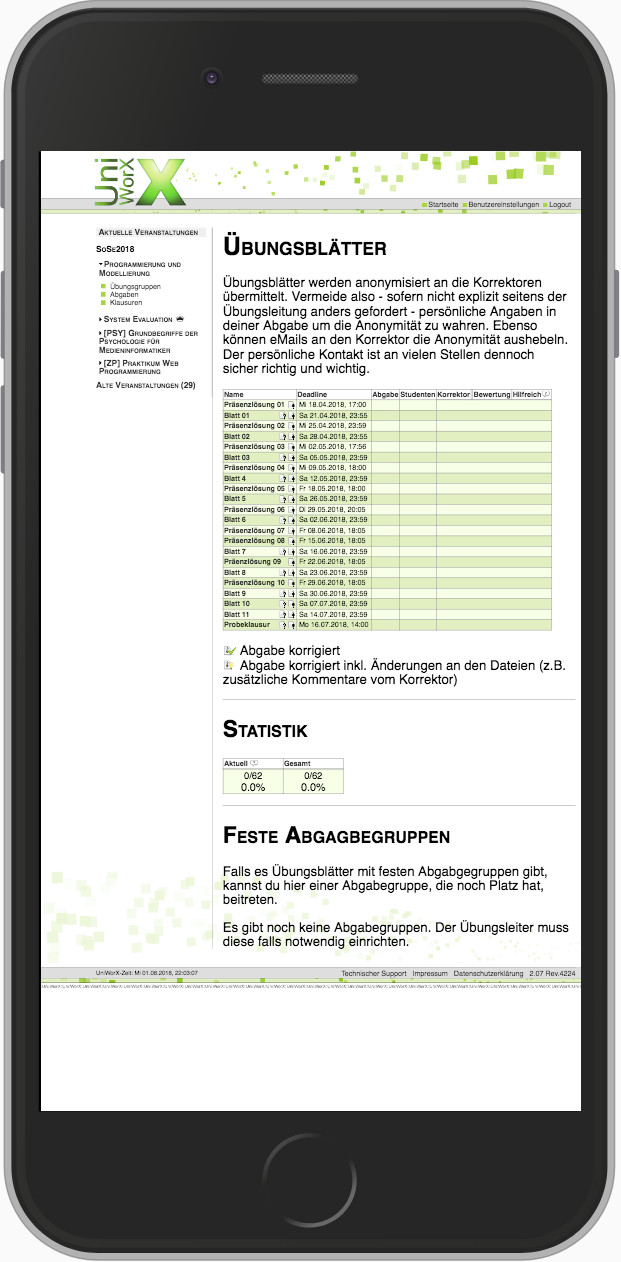
\includegraphics[width=67mm]{m_uniworx_sheets.jpg}
      \caption{UniWorX}
      \label{fig:sub1}
    \end{subfigure}%
    \begin{subfigure}{.5\textwidth}
      \centering
      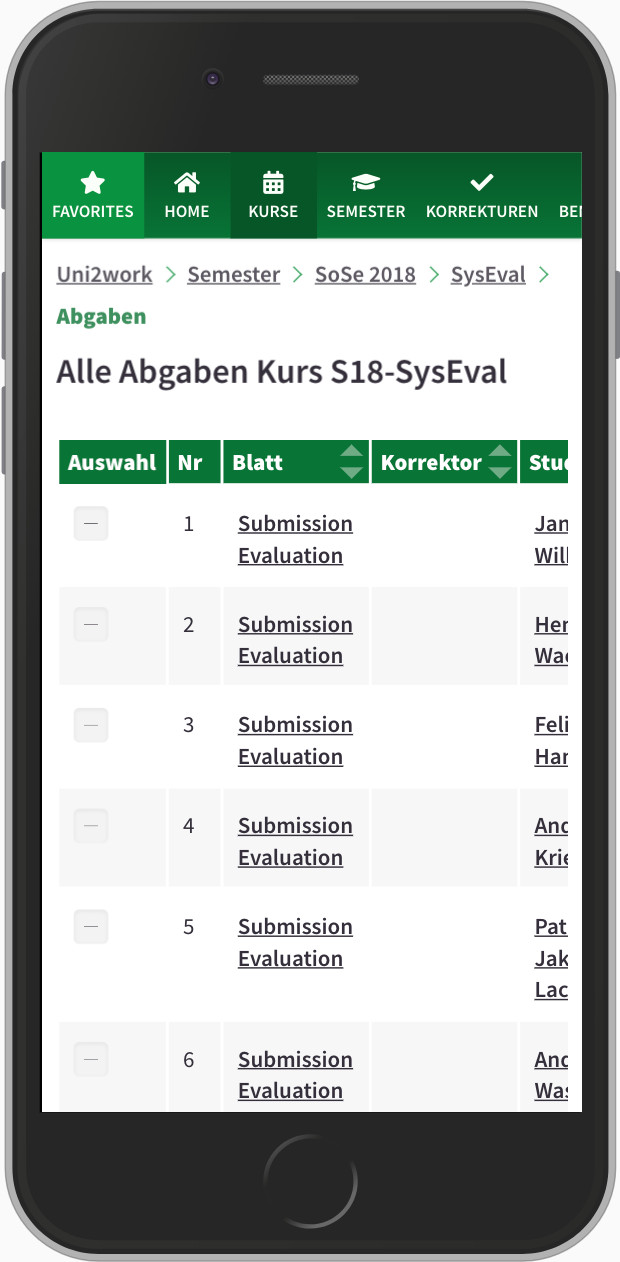
\includegraphics[width=67mm]{m_uni2work_sheets_green.jpg}
      \caption{Uni2work}
      \label{fig:sub2}
    \end{subfigure}
    \caption{Vergleich beider Systeme auf einem Iphone 6/7}
    \label{fig:mobile_comparison}
\end{figure}

\begin{figure}
    \centering
    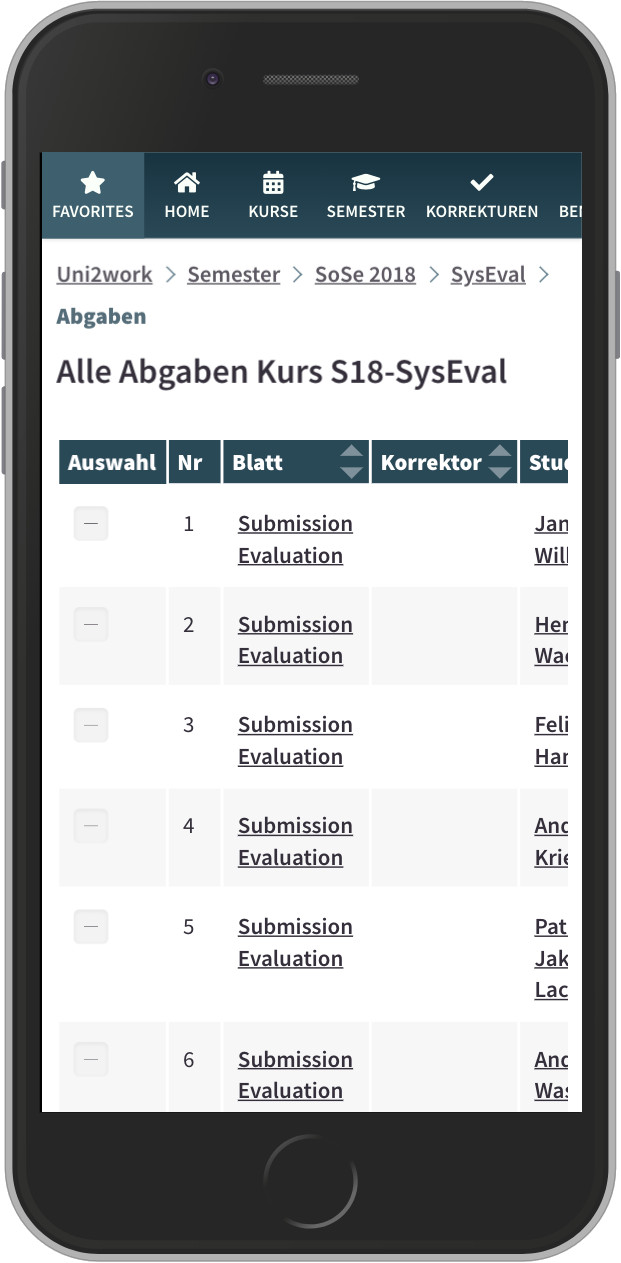
\includegraphics[width=67mm]{m_uni2work_sheets_blue.jpg}
    \caption{Uni2work, Übungsblätter-Übersicht auf Iphone 6}
    \label{fig:uniworx_mobile}
\end{figure}

\begin{figure}
    \centering
    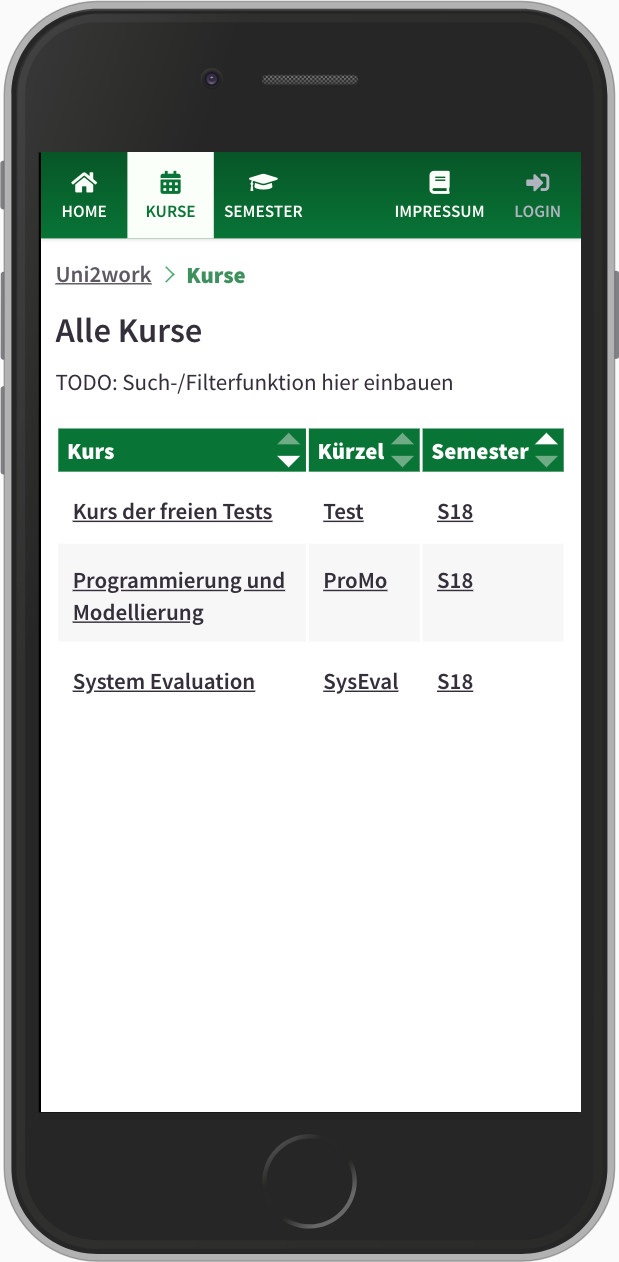
\includegraphics[width=67mm]{m_uni2work_courses_green.jpg}
    \caption{Uni2work, Übungsblätter-Übersicht auf Iphone 6}
    \label{fig:uniworx_mobile}
\end{figure}

Es wurde bei dem Design des \emph{User Interfaces} (\emph{UI}) von Uni2work angenommen, dass sich das Verhalten der Benutzer auf mobilen Geräten grundsätzlich von dem Verhalten der Desktop-Benutzer unterscheidet. 

\clearpage
\section{Studie \& Methode} \label{sec:userstudies}
In der Zeit vom 01.07.2018 bis zum 24.07.2018 wurde eine Studie in Form eines Online-Fragebogens in englischer Sprache durchgeführt.
Das Ziel des Studie war es die Bedienbarkeit (\emph{Usability}) von UniWorX und Uni2work zu evaluieren um einerseits auf die Kritik an UniWorX eingehen und andererseits frühe Fehler in Uni2work vermeiden zu können. Als Plattform für die Einrichtung und Verbreitung des Fragebogens wurde Google Forms gewählt. Der Fragebogen wurde im angegebenen Zeitraum 146 mal ausgefüllt.

Unter den gesammelten Beobachtungen ließen sich vier identifizieren die für die weitere Analyse entfernt wurden, da sie jegliches qualitatives Feedback vermissen ließen und auf alle gestellten Fragen mit der gleichen Antwort reagierten. Eine dieser vier Beobachtungen wurde beim Betrachten der Altersverteilung der Teilnehmer in einem Boxplot identifiziert und bei genauerer Inspektion als irrelevant erkannt, siehe \autoref{fig:participants_age_bp}. Die drei weiteren ausgeschlossenen Beobachtungen offenbarten sich beim manuellen Sichten der Daten.

Bei der Studie handelte es sich um eine \emph{"`within subjects"'}-Studie bei der Teilnehmer der Studie den gleichen Fragebogen auf freiwilliger Basis ein zweites Mal ausfüllen konnten. Die Teilnehmer mussten zu Beginn des Fragebogens eine Aufgabe erfüllen für die sie entweder das bereits vertraute UniWorX (siehe \autoref{sec:uniworx}) oder das neue Uni2work benutzen durften. Ein Teil der anschließenden Fragen bezog sich dann -- soweit nicht anders angegeben -- auf das System das für diese einleitende Aufgabe benutzt wurde. Nach vollständigem Beantworten des Fragebogens wurden die Teilnehmer gebeten den Fragebogen erneut auszufüllen, jedoch bei der initialen Aufgabe das jeweils andere System zu wählen. Den Teilnehmern entstand kein Vorteil durch das zweimalige Ausfüllen des Fragebogens und es wurde nicht erhoben -- und ist nicht mehr nachvollziehbar -- wie viele der Teilnehmer den Fragebogen tatsächlich mehrmals ausgefüllt haben.

Die durch den Fragebogen gesammelten Beobachtungen lassen sich somit in zwei Gruppen aufteilen:

\begin{itemize}
    \item \textbf{Gruppe UniWorX} hat das System \textbf{UniWorX} benutzt und evaluiert.
    \item \textbf{Gruppe Uni2work} hat das System \textbf{Uni2work} benutzt und evaluiert.
\end{itemize}

Diese beiden Gruppen unterscheiden sich somit lediglich in dem System welches für die initiale Aufgabe benutzt wurde, womit \emph{eine unabhängigen Variable} existiert.

\subsection{Likert Skala} \label{sec:likert}
In dem Fragebogen zu dieser Studie wurden manche Fragen in Form der \emph{Likert Skala} gestellt.
Diese Skala bietet eine Möglichkeit die individuelle Einstellung einer Person zu einer Aussage mit einem Wert zu versehen. Bei "`Fragen"' die in der Form der Likert Skala gestellt werden, werden den Teilnehmern Aussagen dargeboten, auf die sie mit einem Wert zwischen "`Widerspreche eindeutig"' (1) und "`Stimme eindeutig zu"' (5) reagieren sollen. Neben dem \emph{System Usability Scale} (s. \autoref{sec:sus}) verwenden auch weitere Fragen des Fragebogens die Likert Skala. Näheres dazu in \autoref{sec:study_structure}.

\subsection{System Usability Scale (SUS)} \label{sec:sus}
Der \emph{System Usability Scale} (SUS) ist eine 1986 von John Brooke vorgestellte Sammlung zehn standardisierter Aussagen \cite{brooke_sus} auf die Studienteilnehmer mit einer Reaktion auf der Likert Skala antworten sollen. Die Reaktionen auf diese zehn Aussagen werden zu einem genormten Wert zwischen 0 und 100 umgerechnet und erlauben somit einen vergleichbaren Messwert der gefühlten Usability eines Systems.

Mit Hilfe des SUS können Systeme Domäne-übergreifend auf ihre Bedienbarkeit untersucht werden indem die enthaltenen Aussagen nicht auf spezielle Funktionalitäten des \emph{System Under Test} (\emph{SUT} -- das System das getestet wird) eingehen, sondern ganz allgemein die Einstellung der Teilnehmer zu generellen Aspekten der Usability messen.

\begin{quote}
\emph{"'[...] there are no absolute measures of usability [...]"'} -- John Brooke, \cite{brooke_sus}
\end{quote}
"`Usability ist nicht in absoluten Werten messbar"'. Mit dieser Aussage unterstreicht der Erfinder des SUS, dass ein einzelner Wert dieser Skala keine Aussagekraft mit sich bringt. Erst der Vergleich mit Werten anderer Systeme die es zu vergleichen gilt bringt einen tatsächlichen Informationsgewinn.

\paragraph{Die zehn standardisierten Aussagen des SUS:}

\begin{itemize}
    \item \textbf{Ich denke ich würde dieses System gerne öfter benutzen} \\ ("'I think that I would like to use this system frequently"')
    \item \textbf{Ich fand das System unnötig komplex} \\ ("'I found the system unnecessarily complex"')
    \item \textbf{Ich fand das System einfach zu benutzen} \\ ("'I thought the system was easy to use"')
    \item \textbf{Ich denke ich würde technische Hilfe in Anspruch nehmen müssen um das System zu benutzen} \\ ("'I think that I would need the support of a technical person to be able to use this system"')
    \item \textbf{Ich fand die verschiedenen Funktionen des Systems waren gut integriert} \\ ("'I found the various functions in this system were well integrated"')
    \item \textbf{Ich fand es gab zu viele Inkonsistenzen in dem System} \\ ("'I thought there was too much inconsistency in this system"')
    \item \textbf{Ich kann mir vorstellen, dass die meisten Menschen den Umgang mit dem System sehr schnell lernen könnten} \\ ("'I would imagine that most people would learn to use this system very quickly"')
    \item \textbf{Ich empfand die Benutzung des Systems als sehr mühsam} \\ ("'I found the system very cumbersome to use"')
    \item \textbf{Ich habe mich sehr sicher beim Umgang mit dem System gefühlt} \\ ("'I felt very confident using the system"')
    \item \textbf{Ich musste viel lernen bevor ich mit dem System umzugehen wusste} \\ ("'I needed to learn a lot of things before I could get going with this system"')
\end{itemize}

\subsection{Studienteilnehmer} \label{sec:studyparticipants}
Bei den Teilnehmern dieser Studie handelte es sich ausschließlich um Besucher der Veranstaltung "`Programmierung und Modellierung"' bei Dr. Steffen Jost im Sommersemester 2018.
Die Teilnehmer der Studie waren im Mittel 22 Jahre alt. Weitere persönliche Daten wurden nicht erfasst.

Der Link zu dem Online-Fragebogen wurde auf einem Übungsblatt des Kurses "`Programmierung und Modellierung"' veröffentlicht. Als Motivation zur Beantwortung des Fragebogens wurden den Teilnehmern Bonuspunkte im Übungsbetrieb gewährt.
Über die genaue Anzahl der Teilnehmer kann keine abschließende Aussage gemacht werden, da nicht erfasst wurde wie viele der Teilnehmer den Fragebogen ein zweites Mal ausgefüllt haben.

\begin{figure}
    \centering
    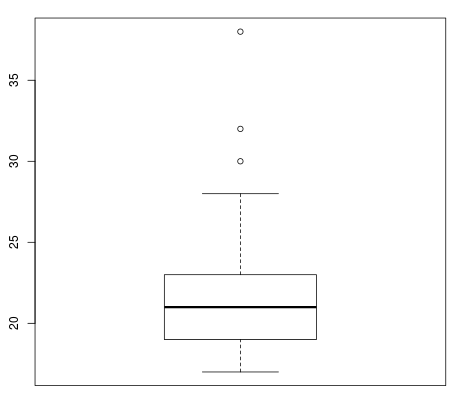
\includegraphics[width=\textwidth]{boxplot_age.png}
    \caption{Alter der Teilnehmer als Boxplot.}
    \label{fig:participants_age_bp}
\end{figure}

\subsection{Frabogenstruktur} \label{sec:study_structure}
Der Fragebogen war in sieben Sektionen aufgeteilt. Diese sollen hier genauer erläutert werden.

\paragraph{Sektion 1: Generelle Fragen zur Person}
Die Fragen in dieser Sektion sollten den Teilnehmer auf die Situation vorbereiten und langsam an das Befragt-Werden gewöhnen. Die Teilnehmer wurden gebeten ihr Alter und ihre ungefähre Nutzungs-Häufigkeit von UniWorX anzugeben. Da alle Studenten die an der Studie teilgenommen haben zwangsläufig UniWorX für ihren Studienalltag benutzen müssen konnte hier davon ausgegangen werden, dass alle Teilnehmer mit UniWorX vertraut waren.

Auf die Frage \textbf{"`Wie oft benutzen Sie UniWorX ungefähr?"'} konnte mit einer dieser sechs Möglichkeiten geantwortet werden:

\begin{itemize}
    \item \textbf{Einmal pro Semester} \\ ("`Once a term"')
    \item \textbf{Einmal pro Monat} \\ ("`Once a month"')
    \item \textbf{Einmal pro Woche} \\ ("`Once a week"')
    \item \textbf{Bis zu fünf Mal pro Woche} \\ ("`Up to five times a week"')
    \item \textbf{Täglich} \\ ("`Daily"')
    \item \textbf{Andauernd} \\ ("`All the time"')
\end{itemize}

\bigskip
\noindent
Für die Angabe des \textbf{Alters} wurde ein Textfeld dargeboten.

\paragraph{Sektion 2: Task}
In dieser Sektion wurde der Teilnehmer aufgefordert eine Aufgabe zu erledigen und die Beantwortung des Fragebogens erst nach beendeter Durchführung der Aufgabe fortzusetzen.

Die genaue Aufgabenstellung in englischer Sprache lautete 
\begin{quote}
\itshape 
Please complete this task before you proceed with this questionnaire:

Use either UniWorX OR Uni2work to find the course "'System Evaluation"' and register for it!
Once you are registered submit anything for the sheet "'Submission Evaluation"'.

UniWorX: https://uniworx.ifi.lmu.de
Uni2work: https://uni2work.ifi.lmu.de

Continue with this questionnaire afterwards.
\end{quote}

\noindent
Eine freie Übersetzung ins Deutsche:
\begin{quote}
\itshape
Bitte beenden Sie diese Aufgabe bevor Sie mit dem Beantworten des Fragebogens fortfahren:

Benutzen Sie \textbf{entweder} UniWorX \textbf{oder} Uni2work um den Kurs "`System Evaluation"' zu finden und sich für den Kurs zu registrieren.
Wenn Sie sich erfolgreich angemeldet haben laden Sie eine beliebige Datei als Abgabe für das Übungsblatt "`Submission Evaluation"' hoch.

[Links zu den beiden Systemen UniWorX und Uni2work]

Fahren Sie im Anschluß mit der Beantwortung dieses Fragebogens fort.
\end{quote}

\paragraph{Sektion 3: Wahl des Systems}
In dieser Sektion sollte der Teilnehmer lediglich angeben für welches System er sich im vorangegangenen Schritt entschieden hat.

\paragraph{Sektion 4: Usability des Systems}
Je nach dem System welches der Teilnehmer in Sektion 2 gewählt hat, wurde ihm in dieser Sektion ein Fragebogen über die Usability dieses Systems präsentiert. Um die Bedienbarkeit verlässlich zu messen wurden die zehn Aussagen des "`System Usability Scale
(\emph{SUS})"' verwendet. Auf diese Aussagen (z.B. "'I thought the system was easy to use"' -- "`Ich finde das System war einfach zu bedienen"') soll der Teilnehmer mit einem Punkt auf der \emph{Likert Skala} reagieren. Näheres zu dem SUS wird in \autoref{sec:sus} und zur Likert Skala in \autoref{sec:likert} erörtert.

\paragraph{Sektion 5: Spezifischere Fragen zum System}
Nach den stark standardisierten Aussagen des SUS in der vorangegangen Sektion wurden in dieser Sektion etwas spezifischere Aussagen dargeboten die auf die Eigenheiten der Systeme eingehen sollten. Diese vier Aussagen sollten wieder mit Hilfe der Likert Skala beurteilt werden.

\begin{itemize}
    \item \textbf{Ich konnte das System eindeutig der LMU zuordnen} \\ ("'I clearly recognized the system as a part of the LMU"')
    \item \textbf{Ich konnte mich sehr einfach zu einem Kurs anmelden} \\ ("'I was able to register for a course very easily"')
    \item \textbf{Ich konnte das Formular zum Hochladen einer Abgabe schnell finden} \\ ("'I was able to find the form for the sheet submission quickly"')
    \item \textbf{Es war offensichtlich ob meine Aktionen erfolgreich waren} \\ ("'It was very obvious whether or not my actions were successful"')
\end{itemize}

\paragraph{Sektion 6: Freie Meinungen}
Unter dem Titel "'Other opinions"' konnte der Teilnehmer in dieser Sektion seine Meinungen zu dem benutzten System in Text-Form äußern. Es wurden Textfelder für folgende Fragen geboten:

\begin{itemize}
    \item \textbf{Was hat Ihnen \emph{besonders gut} gefallen?} \\ ("'Did you like something in particular?"')
    \item \textbf{Was hat Ihnen \emph{besonders schlecht} gefallen?} \\ ("'Did you dislike something in particular?"')
    \item \textbf{Was würden Sie verbessern?} \\ ("'What would you improve?"')
    \item \textbf{Falls Sie das andere System bereits benutzt haben: Was würden Sie daran verbessern?} \\ ("'You feel like you can contribute something to the other system?"')
\end{itemize}

\noindent
Nach diesen vier Freitext-Fragen wurde der Teilnehmer gefragt ob er ein solches System gerne auch auf mobilen Endgeräten verweden würde. Hat der Teilnehmer auf diese Frage mit "`Nein"' geantwortet so wurde er ans Ende des Fragebogens geleitet.

\paragraph{Sektion 7: Usability auf mobilen Endgeräten (Optional)}
Teilnehmer die in der vorigen Sektion angegeben haben, dass sie an einer Benutzung des Systems auf mobilen Endgeräten interessiert wären wurden hier zu ihrem Verhalten auf diesen Geräten befragt.

\begin{itemize}
    \item \textbf{Wie oft besuchen Sie Webseiten die mit Ihrer Universität in Verbindung stehen auf Ihrem Handy oder ähnlichem Gerät?} \\ ("'How often do you visit university related websites on your phone or a similar mobile device?"') \\
    \emph{Antwortmöglichkeiten:} \\ Gleiche Skala wie in Sektion 1 von "`Einmal pro Monat"' bis "`Andauernd"'
    \item \textbf{Haben Sie UniWorX jemals mit Ihrem Handy besucht?} \\ ("'Did you use UniWorX on your mobile device in the past?"') \\ \emph{Antwortmöglichkeiten:} \\ Ja | Nein | Vielleicht
    \item \textbf{Würden Sie UniWorX mehr benutzen wenn es besser an kleine Bildschirme angepasst wäre?} \\ ("'Would you use UniWorX more often on your mobile device if it was better suited for small screens?"') \\ \emph{Antwortmöglichkeiten:} \\ Ja | Nein | Vielleicht | Habe es nicht benutzt
\end{itemize}

\noindent
Nach diesen Fragen kam eine weitere, optionale Freitext-Frage für besonders engagierte Teilnehmer die mit \textbf{"'Feeling extra helpful?"'} angesprochen wurden. Diese wurden gebeten Uni2work mit einem mobilen Gerät ihrer Wahl zu besuchen, sich dort "`umzusehen"' und dann ihre freie Meinung zu dem System in Text-Form zu äußern.

\clearpage
\section{Ergebnisse}
\subsection{Qualitative Auswertung} \label{sec:results_qualitative}
In Sektion 6 der Studie (siehe \autoref{sec:study_structure}) wurden die Teilnehmer gebeten Ihre Meinungen zu verschiedenen Aspekten in freier Text-Form nieder zu schreiben. 
Unter den Antworten finden sich sowohl konstruktive Verbesserungsvorschläge für UniWorX und Uni2work, als auch einfache Aussagen darüber was den Studenten an den Systemen besonders gut, bzw. besonders schlecht gefallen hat.

Zuerst soll darauf eingegangen werden was den Teilnehmern missfiel:

\paragraph{Dinge die nicht gefallen haben: \textbf{UniWorX}}
\begin{itemize}
    \item Aus der Mode gekommenes Design
    \item Nur Informatik-nahe Veranstaltungen verfügbar
    \item Keine visuelle Verbindung zur LMU
    \item Schlechte Übersichtlichkeit der Veranstaltungen und keine Möglichkeit der Suche / Filterung
\end{itemize}

\paragraph{Dinge die nicht gefallen haben: \textbf{Uni2work}}
\begin{itemize}
    \item Nicht ersichtlich ob bereits eine Abgabe für ein Übungsblatt hochgeladen wurde in der Übungsblatt-Übersicht
\end{itemize}

Viele der Antworten der Studenten enthielten konkrete Verbesserungsvorschläge:

\paragraph{Verbesserungsvorschläge: \textbf{UniWorX}}
\begin{itemize}
    \item Performanz - vor allem bei Seiten mit langen Listen
    \item Verfügbarkeit der Materialien eines Kurses über UniWorX
    \item Leichter verständliche Klausur-Anmeldungen (-staTUSSE)
    \item Sortierung von Veranstaltungen nach Abschluss, Studiengang, Fakultät, Prüfungsordnung, etc.
    \item Suchleiste für Kurse
    \item Verwendbarkeit auf kleinen Bildschirmen
    \item Automatisch generierter Stundenplan
    \item Einfachere Anzeige vergangener Kurse
\end{itemize}

\paragraph{Verbesserungsvorschläge: \textbf{UniWorX}}
\begin{itemize}
    \item Übersichtlichtere Kurs-Seiten
    \item Besser erkennbare Statusmeldungen und Rückmeldungen des Systems (Success, Error, etc.)
    \item Farbliche Hinweise auf die Dringlichkeit einer Abgabe (rot wenn <24h)
    \item Eine Klausuren-Seite als Element der Hauptnavigation
    \item Drag & Drop für Dateiuploads
\end{itemize}

In Sektion 7 des Fragebogens (siehe \autoref{sec:study_structure}) wurde nach Meinungen zur Usability auf Geräten mit kleinen Bildschirmen gefragt. Die Rückmeldungen waren überwiegend positiv. Mehrere Studenten haben jedoch angemerkt, dass Tabellen die breiter als der Bildschirm sind zwar mit horizontalem Scrollen betrachtet werden können, sich jedoch womöglich eine andere Form der Darstellung finden ließe mit der kein Scrollen notwendig wäre. Konkrete Ideen dazu wie eine solche Darstellung aussehen könnte waren in den Antworten nicht enthalten, wird aber definitiv bei der nächsten Ideenfindungs-Phase berücksichtigt werden.

\subsection{System Usability Scale (SUS)} \label{sec:results_sus}
Die Ergebnisse der Reaktionen auf die SUS-Aussagen lässt sich für einen ersten Überblick visuell darstellen. In \autoref{fig:results_sus} sind die Reaktionen der Benutzer beider System gegenübergestellt. Die Verteilungen der Reaktionen stimmen bei beiden System weitestgehend überein, bei UniWorX ist jedoch ein leicht ausgeprägterer Trend zu den Rändern hin erkennbar. Reaktionen abseits der Mitte waren auf die Aussagen 1, 2, 3, 6, 7 und 9 für UniWorX extremer als für Uni2work.

Der aus den Reaktionen berechnete SUS-Wert offenbart für das bestehende System UniWorX eine etwas bessere Usability (82,27) als für Uni2work (76,8).
Bangor et al. versuchten nach langjährigem Einsatz des SUS die resultierenden Werte von 0 bis 100 auf eine Skala Menschen-verständlicher Adjektive zu übertragen \cite{bangor_sus_adjective}. Auf dieser Skala von Bangor et al. bewegen sich beide Systeme im Bereich zwischen "`Gut"' und "`Exzellent"'.

\begin{figure}
    \centering
    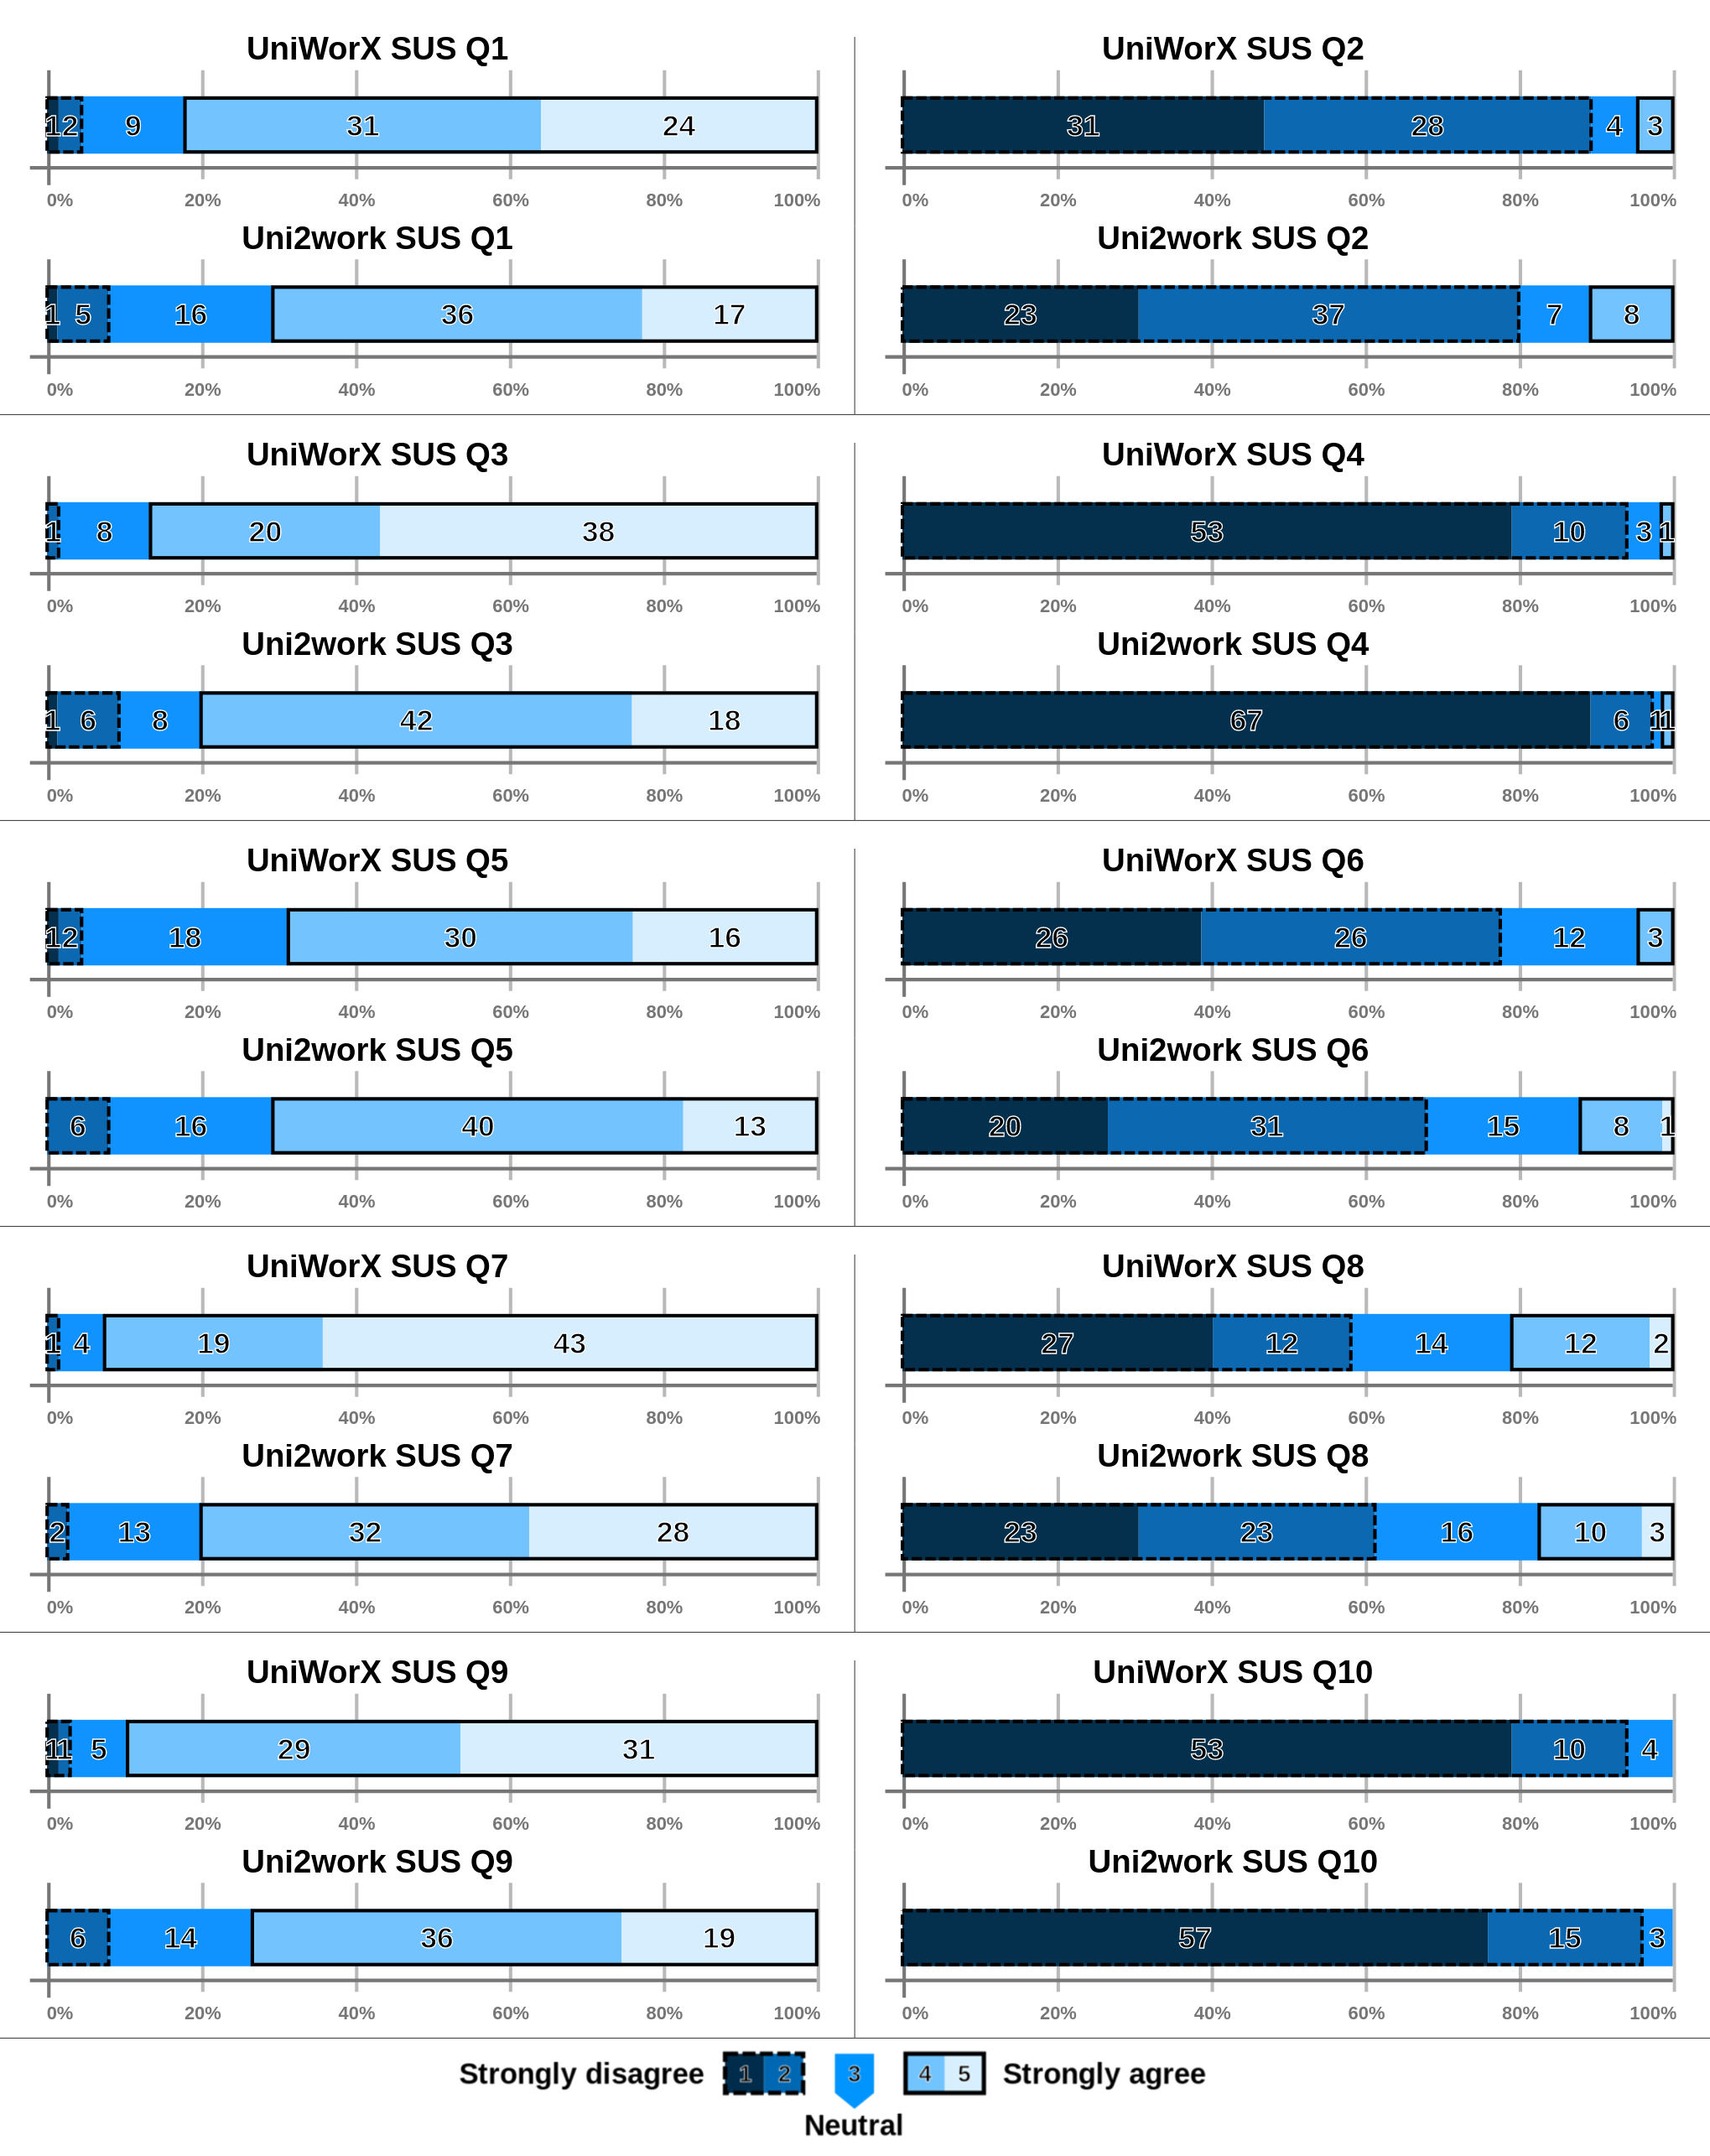
\includegraphics[width=\textwidth]{likert_comparison.jpg}
    \caption{Vergleich der SUS-Reaktionen}
    \label{fig:results_sus}
\end{figure}

\subsection{Likert scale questions} \label{sec:results_likert}

\subsection{Discussion} \label{sec:results_discussion}
Interpretation. What did we learn?
Being used to the old system benefits the scores

4 / 5 outcomes, take away message as a guide for the "next gen"

\clearpage
\section{Rückblick und Ausblick}
Summary, Follow-up work

Zwei Teile blabla

\clearpage
\section*{Useful snippets}
This section just to collect snippets for maybe later use

\begin{center}
	\begin{tabular}{ m{10em} m{10cm} } 
		Participating actor  & Initiated by dormitory resident\\ 
		\hline
		Flow of events &
		\begin{enumerate}
			\item The resident opens the Announcement Wall.
			\item The Announcement Wall displays a list of announcements.
			\item The resident selects „New Announcement“.
			\item The Announcement Wall displays a menu to add a new announcement.
			\item The DormitoryResident fills in their announcement details, selects the “add vote” option and clicks „ADD“.
			\item The Announcement Wall displays the new announcement.
		\end{enumerate}	
		\\ 
		\hline
		Entry condition & The resident has an account and is logged in into the platform.\\ 
		\hline
		Exit condition & The new announcement is saved and displayed on the Announcement Wall. \\ 
		\hline
		Quality requirements & All changes on the Announcement Wall are immediately visible to all residents.
	\end{tabular}
\end{center}

%\_____________________________________________________________________

\cleardoublepage
\section{Zusammenfassung}
TBD

\cleardoublepage
\fancyhead[LE,RO,LO,RE]{} % Keine Kopfzeile mehr oben auf jeder Seite
\section*{Inhalt der beigelegten CD}
%______________________________________________________________________

\cleardoublepage
\bibliographystyle{unsrt}
\bibliography{literature}

\end{document}
